\chapter{Формы}

Мы уже упоминали граничное условие: если данные приходят в приложение или покидают его,
мы должны их проверять. Вероятно, наиболее сложная проверка происходит в формах.
Программировать формы не так просто; в идеальных условиях мы хотели бы уметь:

\begin{itemize}
\item убеждаться, что данные корректны;
\item преобразовать строковые данные формы в типы данных Haskell; % FIXME: marshal --- ?
\item генерировать код HTML для отображения формы;
\item генерировать Javascript, выполняющий валидацию на стороне клиента и предоставляющий
более дружелюбные виджеты, такие как, например, выбор даты;
\item строить более сложные формы, объединяя вместе более простые;
\item автоматически присваивать полям имена, для которых гарантируется уникальность.
\end{itemize}

Пакет \lstinline'yesod-form' предоставляет все эти возможности с простым декларативным
API. Формы строятся из виджетов Yesod для упрощения дизайна форм и последующего применения
Javascript. Здесь, как и везде в Yesod, для обеспечения
корректной работы используется система типов Haskell.
% FIXME: styling (of forms) --- дизайн (форм)

\section{Краткий обзор}

% FIXME: род i18n --- женский (интернационализация?)
\begin{lstlisting}
{-# LANGUAGE QuasiQuotes, TemplateHaskell, MultiParamTypeClasses,
    OverloadedStrings, TypeFamilies #-}
import Yesod
import Yesod.Form.Jquery
import Data.Time (Day)
import Data.Text (Text)
import Control.Applicative ((<$>), (<*>))

data Synopsis = Synopsis

mkYesod "Synopsis" [parseRoutes|
/ RootR GET
/person PersonR POST
|]

instance Yesod Synopsis

-- Указывает приложению использовать стандартные английские сообщения
-- Если вам нужна i18n, вы можете предоставить функцию перевода
instance RenderMessage Synopsis FormMessage where
    renderMessage _ _ = defaultFormMessage

-- И указывает, где найти библиотеки jQuery. Мы будем использовать значение
-- по умолчанию, указывающее на Google CDN
instance YesodJquery Synopsis

-- Тип данных, который мы хотим получить из формы
data Person = Person
    { personName :: Text
    , personBirthday :: Day
    , personFavoriteColor :: Maybe Text
    , personEmail :: Text
    , personWebsite :: Maybe Text
    }
  deriving Show

-- Объявление формы. Сигнатура типа несколько пугающая, но вот её обзор:
--
-- * Параметр Html используется для кодирования некоторой дополнительной
-- информации. См. обсуждение runFormGet и runFormPost ниже для 
-- дополнительного объяснения
--
-- * Как обычно, у нас есть типы под- и главного сайта (FIXME: ХРЕНЬ)
--
-- * FormResult может находиться в трех состояниях: FormMissing (нет
-- доступных данных), FormFailure (некорректные данные) и FormSuccess
--
-- * Widget --- отображаемая форма для вставки на страницу
--
-- Обратите внимание, что шаблон сайта предоставляет удобный синоним типа
-- Form, так что наша сигнатура может быть переписана как:
-- > personForm :: Form Person
--
-- Для целей обучения лучше видеть полную версию
personForm :: Html -> MForm Synopsis Synopsis (FormResult Person, Widget)
personForm = renderDivs $ Person
    <$> areq textField "Name" Nothing
    <*> areq (jqueryDayField def
        { jdsChangeYear = True -- выпадающий список
        , jdsYearRange = "1900:-5" -- от 1900 года до пятилетней давности
        }) "Birthday" Nothing
    <*> aopt textField "Favorite color" Nothing
    <*> areq emailField "Email address" Nothing
    <*> aopt urlField "Website" Nothing

-- Обработчик GET-запроса отображает форму
getRootR :: Handler RepHtml
getRootR = do
    -- генерируем форму, которую будем отображать
    (widget, enctype) <- generateFormPost personForm
    defaultLayout [whamlet|
<p>The widget generated contains only the contents of the form, not the form tag itself.
So...
<form method=post action=@{PersonR} enctype=#{enctype}>
    ^{widget}
    <p>It also doesn't include the submit button.
    <input type=submit>
|]

-- Обработчик POST-запроса обрабатывает форму. Если обработка успешно 
-- завершилась, он отображает данные переданного человека. Иначе -- снова
-- форму с сообщениями об ошибке.
postPersonR :: Handler RepHtml
postPersonR = do
    ((result, widget), enctype) <- runFormPost personForm
    case result of
        FormSuccess person -> defaultLayout [whamlet|<p>#{show person}|]
        _ -> defaultLayout [whamlet|
<p>Invalid input, let's try again.
<form method=post action=@{PersonR} enctype=#{enctype}>
    ^{widget}
    <input type=submit>
|]

main :: IO ()
main = warpDebug 3000 Synopsis
\end{lstlisting}

\section{Виды форм}
Перед тем, как рассмотреть сами типы данных, начнем с обзора разных видов форм. Имеются
три типа
форм:

\begin{description}
\item[Аппликативные] \hfill \\
Наиболее широко используемые (см. пример выше). Аппликативные формы
позволяют нам объединять сообщения об ошибках друг с другом, сохраняя при этом
декларативный высокоуровневый подход. Более детальную информацию об аппликативном подходе
можно почерпнуть в 
\footnotehref{http://www.haskell.org/haskellwiki/Applicative\_functor}{Haskell-вики}.

\item[Монадические] \hfill \\
Более мощная альтернатива аппликативным. Гибкость достигается за счет несколько большей
многословности. Бывают полезны, если необходимо создать форму, которая не укладывается в
стандартный двухстолбцовый формат.

\item[Для ввода] \hfill \\
Используются только для ввода данных. Не генерируют никакого HTML для получения ввода
пользователя. Полезны для взаимодействия с уже существующими формами.
\end{description}


К тому же, существует некоторое число переменных для каждого вида формы и поля,
которые вам, возможно, захочется установить:
\begin{itemize}
\item Поле обязательное или опциональное?
\item Данные должны передаваться методом GET или POST?
\item У поля есть значение по-умолчанию или нет?
\end{itemize}

Основная задача заключается в том, чтобы минимизировать число определений полей и
позволить
им быть полезными в как можно большем числе контекстов. В следствие этого мы добавляем
несколько слов для каждого поля. В обзоре, вы, наверное, заметили такие слова как
\lstinline'areq' и лишний параметр \lstinline'Nothing'. В рамках данной главы мы обсудим 
зачем они нужны, а сейчас можете пока считать, что сделав эти поля явными, мы можем
переиспользовать атомарные(individual) поля (как, например, 
\footnotehref{http://hackage.haskell.org/packages/archive/yesod-form/latest/doc/html/Yesod-Form-Fields.html\#v:intField}
{\lstinline'intField'}) несколькими различными способами.

Замечание по поводу именования. Каждая форма имеет однобуквенный префикс (A, M или I)
который используется в нескольких местах, как например в \lstinline'MForm'. Мы также
будем использовать \lstinline'req' и \lstinline'opt' для обозначения обязательности и
опциональности соответственно. Так мы можем создавать обязательное аппликативное поле с
помощью \lstinline'areq' или опциональное поле для вода данных и помощью \lstinline'iopt'.

\section{Типы}

Модуль \footnotehref{http://hackage.haskell.org/packages/archive/yesod-form/latest/doc/html/Yesod.Form.Types.html}{\lstinline'Yesod.Form.Types'} 
определяет несколько типов. Давайте начнем с самых простых:

\begin{description}
\item[Enctype] \hfill \\
Тип кодировки: либо \lstinline'UrlEncoded', либо \lstinline'Multipart'. Этот тип данных
имеет экземпляр для монады \lstinline'ToHtml', так что вы можете его использовать
непосредственно в \lstinline'Hamlet'-ах.

\item[Env] \hfill \\
Отображает имя параметра в список значений.

\item[FileEnv] \hfill \\
Отображает имя параметра в соответствующий загруженный файл.

\item[Ints] \hfill \\
Как было сказано во введении, формы в Yesod автоматически генерируют уникальные имена 
каждому полю. \lstinline'Ints' используется для хранения этой информации.

\item[FormResult] \hfill \\
Имеет три состояния: \lstinline'FormMissing' если данные не были переданы,
\lstinline'FormFailure' если произошла ошибка при разборе формы (например, отсутствует
обязательное поле или неправильное содержимое) или \lstinline'FormSuccess', когда всё прошло
гладко.
\end{description}

Три следующих типа данных используются для определения индивидуальных
\marginpar{Не нравится мне этот термин, но пока не придумал замену. Может быть
``атомарных''?} полей.

\begin{remark}
Полем называется атомарная часть информации, такая как число, строка или адрес
email. Поля, соединяясь друг с другом, образуют форму.
\end{remark}

\begin{description}
\item[Field] \hfill \\
Определяют два вида функциональности: как преобразовать текстовый вход от пользователя 
в значение языка Haskell и как создавать виджет, который будет показан пользователю.
Несколько атомарных полей пакета \lstinline'yesod-form' определено в модуле
\footnotehref{http://hackage.haskell.org/packages/archive/yesod-form/latest/doc/html/Yesod.Form.Fields.html}{\lstinline'Yesod.Form.Fields'} .

\item[FieldSettings] \hfill \\
Основная информация о том, как поле следует отображать, например: отображаемое имя,
подсказка, и, возможно, захардкоженные ID и имя атрибута. (Если ничего не указано, то они
генерируются автоматически.)

\begin{remark}
\lstinline'FieldSettings' предоставляет экземпляр \lstinline'IsString', так что, 
когда вам понадобится указать значение типа \lstinline'FieldSettings', вы можете 
обойтись просто строковым литералом. Так мы делали во введении.
\end{remark}

\item[FieldView] \hfill \\
Промежуточный формат, содержащий кучу информации о том, как отображать поле. 
Навряд ли это когда-либо понадобится пользователю, мы поговорим об этом позже.
\end{description}


Наконец, мы добрались к важной части нашего рассказа: непосредственно к формам. Существует
три типа форм: \lstinline'MForm' для монадических, \lstinline'AForm' для аппликативных и
\lstinline'IForm' (определенная в 
\footnotehref{http://hackage.haskell.org/packages/archive/yesod-form/latest/doc/html/Yesod-Form-Input.html\#t:IForm}{\lstinline'IForm'}) 
для форм ввода данных. \lstinline'MForm' часто является синонимом типа стека 
монад, который позволяет следующие действия:

\begin{itemize}
\item Монада \lstinline'Reader' предосталяет нам параметры (\lstinline'Env' и 
\lstinline'FileEnv'), the master site argument\marginpar{ммм?} и список языков, 
которые поддерживаются на
стороне пользователя. Последние два используются в \lstinline'i18n', но об это позже.

\item Монада \lstinline'Writer' заботится об \lstinline'Enctype'. Форма всегда будет 
закодирована как  \lstinline'UrlEncoded', за исключением случая, когда присутствует
параметр для загрузки файлов. Тогда у нас форма будет закодирована с помощью multipart.
\item Монада \lstinline'State' хранит \lstinline'Ints' для обеспечения возможности
сгенерировать следующее уникально имя.
\end{itemize}
Форма \lstinline'AForm' устроена сходно. Однако, есть несколько важных различий:
\begin{itemize}
\item Она генерирует список \lstinline'FieldViews'. Это позволяет нам оперировать
абстракцией отображения форм, выбирая соответствующую функцию для отрисовки страницы в
самом конце. Во введении мы использовали \lstinline'renderDivs', которая создает
много тегов \lstinline'div'. Другим вариантом могла бы быть 
\lstinline'renderTable'.

\item У неё нет экземпляра \lstinline'Monad'. Задача \lstinline'Applicative' заключается
в том, чтобы позволить форме выполниться целиком, собрать как можно больше информации, и
выдать результат. Она не может работать в контексте \lstinline'Monad'.
\end{itemize}
\lstinline'IForm' ещё проще: она возвращает либо список ошибок, либо результат.

\section{Преобразование}
"Погодите-ка," скажете вы. "Вы говорите, что во введении использовались аппликативные
формы, но я уверен в том, что сигнатуры типов были \lstinline'MForm'. Не были ли
они монадическими?" Да, верно, в конце сгенерировались монадические формы, но в
действительности они получились преобразованием из аппликативных.

Опять же, наша цель заключается в том, чтобы переиспользовать как можно больше кода и
минимизировать число функций в API. И монадические формы являются более
выразительными, чем аппликативные. Грубо говоря, всё что может быть выражено
аппликативными формами может быть выражено и монадическими. В этом нам помогут две
основные функции: \lstinline'aformToForm' преобразует любую аппликативную форму в
монадическую, а \lstinline'formToAForm' преобразует несколько видов монадических форм в их
аппликативные варианты.

<<Ещё минутку>>, скажете вы. <<Я не видел никаких aformToForm!>> Это тоже верно.
Преобразование произошло в функции \lstinline'renderDivs'.

\section{Создание аппликативных форм}
Теперь, когда (я надеюсь) мы убедились в том, что во введении мы работали с
аппликативными формами, давайте поймем как они создавались. Начнем с простого примера:

\begin{lstlisting}
data Car = Car
    { carModel :: Text
    , carYear :: Int
    }
  deriving Show

carAForm :: AForm Synopsis Synopsis Car
carAForm = Car
    <$> areq textField "Model" Nothing
    <*> areq intField "Year" Nothing

carForm :: Html -> MForm Synopsis Synopsis (FormResult Car, Widget)
carForm = renderTable carAForm

getCarR :: Handler RepHtml
getCarR = do
    ((result, widget), enctype) <- runFormGet carForm
    case result of
        FormSuccess car -> defaultLayout [whamlet|<p>#{show car}|]
        _ -> defaultLayout [whamlet|
<form method=get action=@{CarR} enctype=#{enctype}>
    <table>
        ^{widget}
    <input type=submit>
|]
\end{lstlisting}
Здесь мы явно разделили аппликативные и монадические формы. В \lstinline'carAForm' мы
использовали операторы \lstinline'<$>' и \lstinline'<*>'. Нечему удивляться, они
часто используются при аппликативном программировании. У нас по одной строчке для
каждой записи в типе \lstinline'Car'. Вероятно вы не удивилены тем, что мы использовали 
\lstinline'textField' для записи типа \lstinline'Text' и \lstinline'intField' для записи
типа \lstinline'Int'.

Давайте взглянем поближе на функцию \lstinline'areq'. Её (упрощенной) сигнатурой является
\lstinline'Field a -> FieldSettings -> Maybe a -> AForm a'. 
Первый аргумент определяет тип данных поля, как его разбирать и как отрисовывать.
Следующий аргумент, \lstinline'FieldSettings', дает нам метку, подсказку, имя и  ID
поля. В этом случае мы испльзуем раннее упомянутый экземпляр \lstinline'IsString' для 
\lstinline'FieldSettings'.

А что с \lstinline'Maybe a'? Она предоставляет опциональное значение по умолчанию. 
Например, если мы хватим заполнить форму с помощью <<2007>> как годом машины по
умолчанию, мы воспользуемся \lstinline'areq intField "Year" (Just 2007)'. Мы можем даже
сделать это выше уровнем, так как форма принимает опциональный аргумент для значений по
умолчанию.

\begin{lstlisting}[caption={Формы со значениями по умолчанию}]
carAForm :: Maybe Car -> AForm Synopsis Synopsis Car
carAForm mcar = Car
    <$> areq textField "Model" (carModel <$> mcar)
    <*> areq intField "Year" (carYear <$> mcar)

carForm :: Html -> MForm Synopsis Synopsis (FormResult Car, Widget)
carForm = renderTable (carAForm $ Just $ Car "Forte" 2010)

getCarR :: Handler RepHtml
getCarR = do
    ((result, widget), enctype) <- runFormGet carForm
    case result of
        FormSuccess car -> defaultLayout [whamlet|<p>#{show car}|]
        _ -> defaultLayout [whamlet|
<form method=get action=@{CarR} enctype=#{enctype}>
    <table>
        ^{widget}
    <input type=submit>
|]
\end{lstlisting}

\subsection{Опциональные поля}
Предположим, что нам нужно опциональное поле (например цвет машины). Всё что нужно ---
это воспользоваться функцией \lstinline'aopt'.
\begin{lstlisting}[caption={Опциональные поля}]
data Car = Car
    { carModel :: Text
    , carYear :: Int
    , carColor :: Maybe Text
    }
  deriving Show

carAForm :: AForm Synopsis Synopsis Car
carAForm = Car
    <$> areq textField "Model" Nothing
    <*> areq intField "Year" Nothing
    <*> aopt textField "Color" Nothing

carForm :: Html -> MForm Synopsis Synopsis (FormResult Car, Widget)
carForm = renderTable carAForm

getCarR :: Handler RepHtml
getCarR = do
    ((result, widget), enctype) <- runFormGet carForm
    case result of
        FormSuccess car -> defaultLayout [whamlet|<p>#{show car}|]
        _ -> defaultLayout [whamlet|
<form method=get action=@{CarR} enctype=#{enctype}>
    <table>
        ^{widget}
    <input type=submit>
|]
\end{lstlisting}
Как и в случае обязательных полей, последним аргументом является значение по умолчанию.
Однако, оно завернуто в тип \lstinline'Maybe' два раза. Это может показаться чрезмерным,
но оно урощает написаное кода, который принимает в параметре формы опциональное значение
по умолчанию, как в следующем примере.

\begin{lstlisting}[caption={Опциональные поля по умолчанию}]
data Car = Car
    { carModel :: Text
    , carYear :: Int
    , carColor :: Maybe Text
    }
  deriving Show

carAForm :: Maybe Car -> AForm Synopsis Synopsis Car
carAForm mcar = Car
    <$> areq textField "Model" (carModel <$> mcar)
    <*> areq intField  "Year"  (carYear  <$> mcar)
    <*> aopt textField "Color" (carColor <$> mcar)

carForm :: Html -> MForm Synopsis Synopsis (FormResult Car, Widget)
carForm = renderTable $ carAForm $ Just $ Car "Forte" 2010 $ Just "gray"

getCarR :: Handler RepHtml
getCarR = do
    ((result, widget), enctype) <- runFormGet carForm
    case result of
        FormSuccess car -> defaultLayout [whamlet|<p>#{show car}|]
        _ -> defaultLayout [whamlet|
<form method=get action=@{CarR} enctype=#{enctype}>
    <table>
        ^{widget}
    <input type=submit>
|]
\end{lstlisting}

\section{Валидация}
Как бы сделать так, чтобы наша форма принимала только машины, созданные после 1990 года?
Если вы помните, мы говорили выше, что \lstinline'Field' сам по себе содержит информацию 
о допустимых значениях. Так что, всё что нам надо это использовать новый
\lstinline'Field', верно же? Да, но это будет несколько утомительно. Вместо этого,
давайте изменим уже существующее.
\begin{lstlisting}
carAForm :: Maybe Car -> AForm Synopsis Synopsis Car
carAForm mcar = Car
    <$> areq textField    "Model" (carModel <$> mcar)
    <*> areq carYearField "Year"  (carYear  <$> mcar)
    <*> aopt textField    "Color" (carColor <$> mcar)
  where
    errorMessage :: Text
    errorMessage = "Your car is too old, get a new one!"

    carYearField = check validateYear intField

    validateYear y
        | y < 1990 = Left errorMessage
        | otherwise = Right y

carForm :: Html -> MForm Synopsis Synopsis (FormResult Car, Widget)
carForm = renderTable $ carAForm $ Just $ Car "Forte" 2010 $ Just "gray"

getCarR :: Handler RepHtml
getCarR = do
    ((result, widget), enctype) <- runFormGet carForm
    case result of
        FormSuccess car -> defaultLayout [whamlet|<p>#{show car}|]
        _ -> defaultLayout [whamlet|
<form method=get action=@{CarR} enctype=#{enctype}>
    <table>
        ^{widget}
    <input type=submit>
|]
\end{lstlisting}

Трюк кроется в функции провеки \lstinline'check'. Она принимает функцию 
(\lstinline'validateYear'), которая возвращает либо сообщение об ошибке, либо новое
значение. В этом примере, мы вообще не модифицировали значение, это самый частый случай
использования. И так как этот вид проверки довольно распространён, мы можем применить
сокращение:

\begin{lstlisting}
carYearField = checkBool (>= 1990) errorMessage intField
\end{lstlisting}

\begin{lstlisting}
carForm :: Html -> MForm Synopsis Synopsis (FormResult Car, Widget)
carForm = renderTable $ carAForm $ Just $ Car "Forte" 2010 $ Just "gray"

getCarR :: Handler RepHtml
getCarR = do
    ((result, widget), enctype) <- runFormGet carForm
    case result of
        FormSuccess car -> defaultLayout [whamlet|<p>#{show car}|]
        _ -> defaultLayout [whamlet|
<form method=get action=@{CarR} enctype=#{enctype}>
    <table>
        ^{widget}
    <input type=submit>
|]
\end{lstlisting}

Функция \lstinline'checkBool' принимает два параметра: условие, которое должно быть
выполнено, и сообщение об ошибке, которое следует отобразить, если условие не верно.
\begin{remark}
Вы могли заметить явное указание \lstinline'Text' в сигнатуре типа функции
\lstinline'errorMessage'. При использовании \lstinline'OverloadedStrings' это
необходимо. Чтобы поддерживать i18n, сообщения могут иметь много различных типов
данных и GHC никак не может сам определить, который экземпляр \lstinline'IsString' вам
нужен.
\end{remark}
Классно, что мы можем быть уверены, что наша машина не очень стара. Но что, если мы хотим
быть уверенными в том, что указанный год не из будущего? Чтобы получить текущий год, нам
надо выполнить немного IO. Для таких случаев предназначение функция \lstinline'checkM':

\begin{lstlisting}
    carYearField = checkM inPast $ checkBool (>= 1990) errorMessage intField

    inPast y = do
        thisYear <- liftIO getCurrentYear
        return $ if y <= thisYear
            then Right y
            else Left ("You have a time machine!" :: Text)
\end{lstlisting}

\begin{lstlisting}
getCurrentYear :: IO Int
getCurrentYear = do
    now <- getCurrentTime
    let today = utctDay now
    let (year, _, _) = toGregorian today
    return $ fromInteger year

carForm :: Html -> MForm Synopsis Synopsis (FormResult Car, Widget)
carForm = renderTable $ carAForm $ Just $ Car "Forte" 2010 $ Just "gray"

getCarR :: Handler RepHtml
getCarR = do
    ((result, widget), enctype) <- runFormGet carForm
    case result of
        FormSuccess car -> defaultLayout [whamlet|<p>#{show car}|]
        _ -> defaultLayout [whamlet|
<form method=get action=@{CarR} enctype=#{enctype}>
    <table>
        ^{widget}
    <input type=submit>
|]
\end{lstlisting}

Функция \lstinline'inPast' вернет результат типа \lstinline'Either'. Однако, она
использует монаду \lstinline'Handler'. Мы используем \lstinline'liftIO getCurrentYear',
чтобы получить текущий год и затем сравнить его с годом, указанным пользователем. Также,
обратите внимание как мы несколько валидаторов построили в цепочку.

\begin{remark}
С тех пор как валидатор \lstinline'checkM' работает в монаде \lstinline'Handler', вы
можете писать тот же код, что используете обычно, теперь и в \lstinline'Yesod'. Это 
особенно полезно при обращении к базам данных, что будет рассмотрено в главе
\hyperref[ch:persistent]{Persistent}.
\end{remark}

\section{Более сложные поля}
Наше поле для ввода цвета довольно приличное, но не очень user-friendly
\marginpar{надо как-то переводить на русский}. В
действительности нам нужен выпадающий список.

\begin{lstlisting}[caption={Выпадающие списки}]
data Car = Car
    { carModel :: Text
    , carYear :: Int
    , carColor :: Maybe Color
    }
  deriving Show

data Color = Red | Blue | Gray | Black
    deriving (Show, Eq, Enum, Bounded)

carAForm :: Maybe Car -> AForm Synopsis Synopsis Car
carAForm mcar = Car
    <$> areq textField "Model" (carModel <$> mcar)
    <*> areq carYearField "Year" (carYear <$> mcar)
    <*> aopt (selectFieldList colors) "Color" (carColor <$> mcar)
  where
    colors :: [(Text, Color)]
    colors = [("Red", Red), ("Blue", Blue), ("Gray", Gray), ("Black", Black)]
    errorMessage :: Text
    errorMessage = "Your car is too old, get a new one!"

    carYearField = checkM inPast $ checkBool (>= 1990) errorMessage intField

    inPast y = do
        thisYear <- liftIO getCurrentYear
        return $ if y <= thisYear
            then Right y
            else Left ("You have a time machine!" :: Text)

getCurrentYear :: IO Int
getCurrentYear = do
    now <- getCurrentTime
    let today = utctDay now
    let (year, _, _) = toGregorian today
    return $ fromInteger year

carForm :: Html -> MForm Synopsis Synopsis (FormResult Car, Widget)
carForm = renderTable $ carAForm $ Just $ Car "Forte" 2010 $ Just Black

getCarR :: Handler RepHtml
getCarR = do
    ((result, widget), enctype) <- runFormGet carForm
    case result of
        FormSuccess car -> defaultLayout [whamlet|<p>#{show car}|]
        _ -> defaultLayout [whamlet|
<form method=get action=@{CarR} enctype=#{enctype}>
    <table>
        ^{widget}
    <input type=submit>
|]
\end{lstlisting}

Функция \lstinline'selectFieldList' принимает список пар. Первый элемент пары --- это
текст, который отобразится пользователю в выпадающем списке, а вторым элементом
является соответствующее значение из \lstinline'Haskell'. Конечно, код выше выглядит
солидно, но мы можем получить тот же результат воспользовавшись экземплярами
\lstinline'Enum' и \lstinline'Bounded', которые GHC автоматически
предоставляет нам.

\begin{lstlisting}[caption={Используя Enum и Bounded}]
data Car = Car
    { carModel :: Text
    , carYear :: Int
    , carColor :: Maybe Color
    }
  deriving Show

data Color = Red | Blue | Gray | Black
    deriving (Show, Eq, Enum, Bounded)

carAForm :: Maybe Car -> AForm Synopsis Synopsis Car
carAForm mcar = Car
    <$> areq textField "Model" (carModel <$> mcar)
    <*> areq carYearField "Year" (carYear <$> mcar)
    <*> aopt (selectFieldList colors) "Color" (carColor <$> mcar)
  where
    colors = map (pack . show &&& id) $ [minBound..maxBound]
    errorMessage :: Text
    errorMessage = "Your car is too old, get a new one!"

    carYearField = checkM inPast $ checkBool (>= 1990) errorMessage intField

    inPast y = do
        thisYear <- liftIO getCurrentYear
        return $ if y <= thisYear
            then Right y
            else Left ("You have a time machine!" :: Text)

getCurrentYear :: IO Int
getCurrentYear = do
    now <- getCurrentTime
    let today = utctDay now
    let (year, _, _) = toGregorian today
    return $ fromInteger year

carForm :: Html -> MForm Synopsis Synopsis (FormResult Car, Widget)
carForm = renderTable $ carAForm $ Just $ Car "Forte" 2010 $ Just Black

getCarR :: Handler RepHtml
getCarR = do
    ((result, widget), enctype) <- runFormGet carForm
    case result of
        FormSuccess car -> defaultLayout [whamlet|<p>#{show car}|]
        _ -> defaultLayout [whamlet|
<form method=get action=@{CarR} enctype=#{enctype}>
    <table>
        ^{widget}
    <input type=submit>
|]
\end{lstlisting}

Промежуток \lstinline'[minBound..maxBound]' предоставляет нам список всех различных
значений типа \lstinline'Color'. Мы можем затем применить \lstinline'map' и 
\lstinline'&&&' (a.k.a, the fan-out operator)\marginpar{щито?}, превращая его в список пар.

Некоторые люди предпочитаю кнопки radio buttons\marginpar{забыл как по-русски} 
выпадающим спискам. К счастью, нам надо только провести одно изменение. Вот пример.

\begin{lstlisting}[caption={Radio buttons}]
data Car = Car
    { carModel :: Text
    , carYear :: Int
    , carColor :: Maybe Color
    }
  deriving Show

data Color = Red | Blue | Gray | Black
    deriving (Show, Eq, Enum, Bounded)

carAForm :: Maybe Car -> AForm Synopsis Synopsis Car
carAForm mcar = Car
    <$> areq textField "Model" (carModel <$> mcar)
    <*> areq carYearField "Year" (carYear <$> mcar)
    <*> aopt (radioFieldList colors) "Color" (carColor <$> mcar)
  where
    colors = map (pack . show &&& id) $ [minBound..maxBound]
    errorMessage :: Text
    errorMessage = "Your car is too old, get a new one!"

    carYearField = checkM inPast $ checkBool (>= 1990) errorMessage intField

    inPast y = do
        thisYear <- liftIO getCurrentYear
        return $ if y <= thisYear
            then Right y
            else Left ("You have a time machine!" :: Text)

getCurrentYear :: IO Int
getCurrentYear = do
    now <- getCurrentTime
    let today = utctDay now
    let (year, _, _) = toGregorian today
    return $ fromInteger year

carForm :: Html -> MForm Synopsis Synopsis (FormResult Car, Widget)
carForm = renderTable $ carAForm $ Just $ Car "Forte" 2010 $ Just Black

getCarR :: Handler RepHtml
getCarR = do
    ((result, widget), enctype) <- runFormGet carForm
    case result of
        FormSuccess car -> defaultLayout [whamlet|<p>#{show car}|]
        _ -> defaultLayout [whamlet|
<form method=get action=@{CarR} enctype=#{enctype}>
    <table>
        ^{widget}
    <input type=submit>
|]
\end{lstlisting}

\section{Выполнение форм}\marginpar{В оригинале --- running. Не уверен, что подобрал качественный термин.}
А теперь воспользуемся нашими формами, чтобы получить некоторый результат. Для этого
существует несколько различных функций, каждая из которых имеет своё назначение. Я
пройдусь по всем, ничиная с самых распространённых.

\subsection{runFormPost}

This will run your form against any submitted POST parameters.
\marginpar{Я ничего не понял} If this is not a POST
submission, it will return a FormMissing. Токен безопасности вставится автоматически
как скрытое поле во избежание 
\footnotehref{http://en.wikipedia.org/wiki/Cross-site\_request\_forgery}{CSRF}-атак.

\subsection{runFormGet}
То же, что и \lstinline'runFormPost' для GET-параметров. Чтобы различать обычную
загрузку страницы через GET от отправки GET формы, она включает дополнительное скрытое
поле \lstinline'_hasdata' в форме.

\subsection{runFormPostNoNonce}
То же, что и \lstinline'runFormPost', но без включения токена безопасности CSRF.

\subsection{generateFormPost}
Вместо связывания существующих POST параметров, действует так, будто их нет. Может
быть полезно когда вам нужно сгенерировать новую форму после того, как предыдущая была
отправлена, such as in a wizard.

\subsection{generateFormGet}
То же, что и \lstinline'generateFormPost', но через GET.

Возвращаемым значением первых трёх является \lstinline'((FormResult a, Widget), Enctype)'.
\lstinline'Widget' уже будет иметь ошибки валидации и предыдущие отправленные значения.
\marginpar{Widget will already have any validation errors and previously submitted values.}

\section{i18n}
Здесь будет просто несколько ссылок к i18n. Эта тема подробнее освещена в своей
собственной  \hyperref[ch:i18n]{главе},
но так как она напрямую связана с формами, я хочу дать краткий обзор. 
Идея по поддержке i18n в Yesod состоит в том, чтобы иметь типы данных для представления
сообщений. Каждый сайт может иметь экземпляр \lstinline'RenderMessage' для конкретного
типа данных, который будет переводить сообщение в сообтветствии со списком языков,
доступных на клиенте. В результате есть несколько вещей, о которых вам стоит знать:
\begin{itemize}
\item  Для каждого сайта автоматически создается экземпляр \lstinline'RenderMessage' для
типа \lstinline'Text', так что вы можете просто использовать простые строки, если не
хотите заботиться о поддержке i18n. Однако, вам неожиданно могут понадобиться явные
сигнатуры типов.
\item Все сообщения в yesod-form выражаются в терминах типа \lstinline'FormMessage'.
Поэтому, для использования yesod-form вам нужен соответствующий экземпляр 
\lstinline'RenderMessage'. Наипростейший, который использует перевод на английский по
умолчанию, будет выглядеть так:
\begin{lstlisting}
instance RenderMessage MyApp FormMessage where
    renderMessage _ _ = defaultFormMessage
\end{lstlisting}
Он предоставляется автоматически шаблоном сайта.
\end{itemize}

\section{Monadic Forms}
Чаще всего необходимо получить формы с простой версткой, и в этом случае аппликативные формы 
вполне справляются. Однако, иногда может понадобиться несколько кастомизированный 
внешний вид форм.

\begin{figure}[tbph]
  \centering
  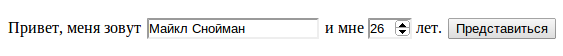
\includegraphics[width=\textwidth]{08-forms-image-01.png}
  \caption{Нестандартный макет формы}
\end{figure}
В таких случаях следует использовать монадические формы. Они несколько более 
многословны чем их аппликативные родственники, но эта многословность позволяет нам
получать полный контроль над тем, как форма будет выглядеть. Чтобы получить такую же
форму, как приведенная выше, мы должны написать что-то подобное этому.

\begin{lstlisting}
{-# LANGUAGE OverloadedStrings, TypeFamilies, QuasiQuotes,
             TemplateHaskell, MultiParamTypeClasses #-}

import Yesod
import Control.Applicative
import Data.Text (Text)

data MFormExample = MFormExample

mkYesod "MFormExample" [parseRoutes|
/ RootR GET
|]

instance Yesod MFormExample

instance RenderMessage MFormExample FormMessage where
    renderMessage _ _ = defaultFormMessage

data Person = Person { personName :: Text, personAge :: Int }
    deriving Show

personForm :: Html -> MForm MFormExample MFormExample (FormResult Person, Widget)
personForm extra = do
    (nameRes, nameView) <- mreq textField "this is not used" Nothing
    (ageRes, ageView) <- mreq intField "neither is this" Nothing
    let personRes = Person <$> nameRes <*> ageRes
    let widget = do
            toWidget [lucius|
##{fvId ageView} {
    width: 3em;
}
|]
            [whamlet|
#{extra}
<p>
    Hello, my name is #
    ^{fvInput nameView}
    \ and I am #
    ^{fvInput ageView}
    \ years old. #
    <input type=submit value="Introduce myself">
|]
    return (personRes, widget)

getRootR :: Handler RepHtml
getRootR = do
    ((res, widget), enctype) <- runFormGet personForm
    defaultLayout [whamlet|
<p>Result: #{show res}
<form enctype=#{enctype}>
    ^{widget}
|]

main :: IO ()
main = warpDebug 3000 MFormExample
\end{lstlisting}
Подобно тому, как мы использовали \lstinline'areq' в аппликативном случае, мы используем 
\lstinline'mreq' в монадическом. 
(И да, также можно использовать \lstinline'mopt' для опциональных полей).
Но здесь есть существенное различие: \lstinline'mreq' выдает нам пару значений. 
Вместо того, чтобы скрываеть значение типа 
\footnotehref{http://hackage.haskell.org/packages/archive/yesod-form/latest/doc/html/Yesod-Form-Types.html\#t:FieldView}{FieldView}
и автоматически вставлять его в виджет, мы получаем возможность вставить его 
туда, куда хотим.

Значение типа \lstinline'FieldView' содержит немало информации. Самой важной является 
\lstinline'fvInput', которая описывает поле формы. В этом примере мы также использовали
\lstinline'fvId', которое содержит HTML id элемента управления для ввода данных. Мы
его использовали для того, чтобы указать ширину поля.

Вы можете заинтересоваться назначением значений "this is not used" и "neither is this".
Функция \lstinline'mreq' принимает вторым аргументом значение типа \lstinline'FieldSettings'.
Так как для \lstinline'FieldSettings' сущетвует экземпляр \lstinline'IsString', такие строки 
по сути раскрываются компилятором в:

\begin{lstlisting}
fromString "this is not used" == FieldSettings
    { fsLabel = "this is not used"
    , fsTooltip = Nothing
    , fsId = Nothing
    , fsName = Nothing
    , fsClass = []
    }
\end{lstlisting}

В случае аппликативных форм, значения \lstinline'fsLabel' и \lstinline'fsTooltip'
использовались при построении HTML. В монадических, Yesod не генерирует для нас
никаких HTML-обёрток и по этой причине эти значения игнорируются. Однако, мы храним 
параметр типа \lstinline'FieldSettings' для того, чтобы мы могли, 
когда нам захочется, переопределять атрибуты id или name у наших полей.

Другим интересным моментом является дополнительное значение. Формы типа GET используют
его, чтобы обозначить, что они были отправлены, а POST формы включают токены безопасности
во избежание 
\footnotehref{http://en.wikipedia.org/wiki/Cross-site\_request\_forgery}{CSRF}-атак. 
Если вы не включите это дополнительное поле, то Yesod не примет вашу форму.

Остальные вещи довольно-таки тривиальны. Мы создаем наше значение типа 
\lstinline'personRes' из значений \lstinline'nameRes' и \lstinline'ageRes', а 
затем возвращаем пару, описывающую человека и виджет. А функции \lstinline'getRootR'
всё происходит так, будто мы используем аппликативные формы. В действительности, вы
можете 
заменить монадическую реализацию формы на аппликативную, а этот код будет всё ещё работать.

\section{Формы ввода данных}
Аппликативные и монадические формы занимаются и генерацией HTML, и разбором данных.
Иногда вам нужно только последнее, например, когда где-то уже создана форма, или если вы
хотите сгененрировать форму динамически, используя Javascript. В этих случаях вам пригодятся
формы ввода данных.

Они похожи на аппликативные и монадические, но есть некоторые различия:
\begin{itemize}
 \item Вы используете \lstinline'runInputPost' и \lstinline'runInputGet'.
 \item Вы используете \lstinline'ireq' и \lstinline'iopt'. Эти функции теперь 
 принимают только 2 аргумента:
 тип поля и его имя (т.е. значение HTML атбрибута name) of the field in question.
 \item После выполнения формы, она возвращает значение. 
 Она не возвращает виджет или тип кодировки.
 \item В случае ошибок проверки данных, страница перенаправится на странцу 
 с сообщением об ошибке <<invalid arguments>>.
\end{itemize}
Вы можете переписать предыдущий пример с помощью форм ввода данных. Однако, стоит 
заметить, что они менее user friendly. Если вы допустите ошибку при заполнении 
аппликативной или монадической формы, то вы будете перенаправлены на ту же 
страницу, где предыдущие введенные данные сохранятся, а сообщение об ошибке 
укажет, что надо справить. Для форм ввода данных пользователей получит только 
сообщение об ошибке.

\begin{lstlisting}
{-# LANGUAGE OverloadedStrings, TypeFamilies, QuasiQuotes,
             TemplateHaskell, MultiParamTypeClasses #-}

import Yesod
import Control.Applicative
import Data.Text (Text)

data Input = Input

mkYesod "Input" [parseRoutes|
/ RootR GET
/input InputR GET
|]

instance Yesod Input

instance RenderMessage Input FormMessage where
    renderMessage _ _ = defaultFormMessage

data Person = Person { personName :: Text, personAge :: Int }
    deriving Show

getRootR :: Handler RepHtml
getRootR = defaultLayout [whamlet|
<form action=@{InputR}>
    <p>
        My name is #
        <input type=text name=name>
        \ and I am #
        <input type=text name=age>
        \ years old. #
        <input type=submit value="Introduce myself">
|]

getInputR :: Handler RepHtml
getInputR = do
    person <- runInputGet $ Person
                <$> ireq textField "name"
                <*> ireq intField "age"
    defaultLayout [whamlet|<p>#{show person}|]

main :: IO ()
main = warpDebug 3000 Input
\end{lstlisting}

\section{Создание пользовательских полей}
Поля, которые встроены в Yesod наверняка покроют большинство ваших нужд по 
работе с формами. Но иногда вам может понадобиться что-то более специализированное.
К счастью, вы можете создавать новые формы в Yesod самостоятельно. Тип данных
\lstinline'Field' имеет две записи. Первая, \lstinline'fieldParse', принимает 
список значений, отправленных пользователем, и возвращает один из трех результатов:
\begin{enumerate}
 \item Сообщение об ошибке в случае, если проверка данных провалилась.
 \item Разобранное значение.
 \item \lstinline'Nothing', сообщая, что данные не были предоставлены.
\end{enumerate}	

Последний случай может несколько удивить: разве Yesod не может автоматически понять,
что информации не было предоставлено, если входной список пуст? Не совсем. Чекбоксы,
например, сообщают о сброшенном состоянии, посылая пустой список.

Also, what's up with the list? \marginpar{Помогайте.} 
Shouldn't it be a Maybe? Well, that's also not the case.
With grouped checkboxes and multi-select lists, you'll have multiple widgets with the same
name. We also use this trick in our example below.

Вторая запись называется \lstinline'fieldView' и она отвечает за отрисовку виджета
пользователю. У этой функции 4 аргумента: атрибут id, атрибут name, результат и булевый флаг, 
для случая, когда поле является обязательным\marginpar{Что-то здесь не так с этим словом}.

Что мы подразумеваем под результатом? В действительности он типа \lstinline'Either'
и выдает либо неразобранные входные данные, когда разбор не удался, либо успешно 
разобранное значение. Великолепный пример этому --- поле \lstinline'intField'.
Если вы введете 42, то в результате будет \lstinline'Right 42'. Но если вы введёте
слово <<turtle>>, результатом будет \lstinline'Left "turtle"'. Это позволит вам
put in a value attribute on your input tag
that will give the user a consistent experience.

В этом маленьком примере вы создадим новое поле для подтверждения пароля. В нём будет
два элемента управления для ввода текста (оба с одним и тем же значением атрибута name)
и он будет возвращать сообщение об ошибке, если пароли не совпадают. Заметьте, что
здесь не указываются атрибуты value для полей ввода, так как нам не нужно пересылать 
на сервер введенный пользователем пароль.

\begin{lstlisting}
passwordConfirmField :: Field sub master Text
passwordConfirmField = Field
    { fieldParse = \rawVals ->
        case rawVals of
            [a, b]
                | a == b -> return $ Right $ Just a
                | otherwise -> return $ Left "Passwords don't match"
            [] -> return $ Right Nothing
            _ -> return $ Left "You must enter two values"
    , fieldView = \idAttr nameAttr _ eResult isReq -> [whamlet|
<input id=#{idAttr} name=#{nameAttr} type=password>
<div>Confirm:
<input id=#{idAttr}-confirm name=#{nameAttr} type=password>
|]
    }

getRootR :: Handler RepHtml
getRootR = do
    ((res, widget), enctype) <- runFormGet $ renderDivs
        $ areq passwordConfirmField "Password" Nothing
    defaultLayout [whamlet|
<p>Result: #{show res}
<form enctype=#{enctype}>
    ^{widget}
    <input type=submit value="Change password">
|]
main :: IO ()
main = warpDebug 3000 Password
\end{lstlisting}

\section{Заключение}

Формы в Yesod делятся на три вида. Аппликативные используются чаще всего, так как
предоставляют красивый интерфейс и простой для использование API. Монадические формы дают
больше возможностей, но их сложнее использовать. Формы ввода данных полезны, когда вам
надо просто принять данные пользователя, не генерируя сложных виджетов.

Из коробки Yesod предоставляет несколько видов полей для форм. Для использования
форм вам придется определиться, какую форму вы хотите и является поле опциональным или
обязательным. Итого мы имеет шесть дополнительных функций: \lstinline'areq', \lstinline'aopt', \lstinline'mreq', \lstinline'mopt', \lstinline'ireq',
и \lstinline'iopt'.

Формы довольно-таки мощны. Они могут автоматически вставлять код на Javascript, чтобы
получаять более красивые элементы управляения, например, для выбора даты из библиотеки 
jQuery. Формы также поддерживают  i18n, так что вы можете расчитывать на большое
сообщество пользователей. А для более специфических надобностей, вы можете привязать
функции валидации данных для конкретных полей, или написать свои с чистого  листа.

